\chaptercustom{5}{Xây dựng hệ thống}  
\setcounter{section}{5}

Chương này trình bày chi tiết quá trình xây dựng hệ thống quản lý cửa hàng cho thuê và bán máy ảnh film \lq\lq TheFilmery\rq\rq, chứng minh rằng thiết kế ở Chương 3 và Chương 4 đã được hiện thực thành hệ thống chạy được. Nội dung bao gồm: môi trường và công cụ phát triển, quy trình chuyển đổi từ thiết kế sang cài đặt, thiết kế giao diện, chạy thử các Use Case chính và đánh giá kết quả.

% ============================================================
\subsection{Môi trường và công cụ phát triển}
% ============================================================

\subsubsection{Môi trường phát triển}

Hệ thống được phát triển và kiểm thử trên môi trường Windows và Linux. Cơ sở dữ liệu và các dịch vụ nền tảng sử dụng Supabase. Lưu ý rằng hệ thống hiện đang được thiết lập để chạy trong môi trường phát triển cục bộ.

\subsubsection{Công nghệ sử dụng}

Hệ thống được xây dựng theo kiến trúc client-server (3 tầng). Dưới đây là chi tiết các công nghệ được sử dụng ở từng tầng:

\begin{table}[H]
	\centering
	\caption{Môi trường và Công nghệ phát triển}
	\begin{tabularx}{\textwidth}{|l|l|X|}
		\hline
		\textbf{Thành phần} & \textbf{Công cụ / Công nghệ} & \textbf{Vai trò} \\
		\hline
		Hệ điều hành phát triển & Windows / Linux & Môi trường lập trình và kiểm thử \\
		\hline
		Frontend & React, Vite, TypeScript & Xây dựng SPA giao diện người dùng \\
		\hline
		UI Framework & TailwindCSS & Thiết kế giao diện responsive \\
		\hline
		State Management & Zustand & Quản lý trạng thái phía client \\
		\hline
		HTTP Client & Axios & Gửi request tới backend API \\
		\hline
		Backend & Node.js, Express, TypeScript & Xử lý logic nghiệp vụ \\
		\hline
		Validation & Zod & Kiểm tra dữ liệu đầu vào \\
		\hline
		Database & Supabase PostgreSQL & Lưu trữ dữ liệu hệ thống \\
		\hline
		Authentication & Supabase Auth, JWT & Xác thực và phân quyền \\
		\hline
	\end{tabularx}
\end{table}

\subsubsection{Cấu trúc module hệ thống}

\begin{table}[H]
	\centering
	\caption{Cấu trúc module cài đặt}
	\begin{tabularx}{\textwidth}{|l|l|X|}
		\hline
		\textbf{Module} & \textbf{Thành phần chính} & \textbf{Use Case liên quan} \\
		\hline
		\texttt{system-auth} & AuthController, AuthService & UC01-UC05 \\
		\hline
		\texttt{profile-logs} & ProfileController, ProfileService & UC06-UC07 \\
		\hline
		\texttt{inventory} & CategoryService, CameraModelService, EquipmentService & UC08-UC12 \\
		\hline
		\texttt{rentals-pos} & BookingController, BookingService & UC13-UC17 \\
		\hline
		\texttt{finance} & TransactionController, TransactionService & UC18 \\
		\hline
		\texttt{banmayfilm} & SaleProductService, SaleOrderService & UC19-UC22 \\
		\hline
		\texttt{customer-crm} & CustomerService & UC22-UC23 \\
		\hline
		\texttt{expenses} & ExpenseService & UC24 \\
		\hline
		\texttt{feedbacks} & FeedbackService & UC25 \\
		\hline
		\texttt{reporting} & ReportingService & UC26-UC27 \\
		\hline
	\end{tabularx}
\end{table}

Quy trình chạy hệ thống trong môi trường phát triển gồm:
\begin{enumerate}
    \item Cài đặt dependencies cho frontend và backend.
    \item Cấu hình biến môi trường kết nối Supabase.
    \item Khởi động backend API server.
    \item Khởi động frontend React/Vite.
    \item Đăng nhập bằng tài khoản thử nghiệm để kiểm tra các phân hệ.
\end{enumerate}

% ============================================================
\subsection{Ánh xạ từ thiết kế sang cài đặt}
% ============================================================

Dựa trên các mô hình phân tích và thiết kế đã trình bày ở Chương 3 và Chương 4, nhóm tiến hành hiện thực hóa hệ thống theo hướng use-case driven. Mỗi Use Case được ánh xạ thành một hoặc nhiều API endpoint ở tầng backend, đồng thời tương ứng với các giao diện thao tác ở tầng frontend và các bảng dữ liệu ở tầng database.

Về mặt kiến trúc, các màn hình React đóng vai trò là lớp biên tiếp nhận thao tác từ người dùng; các Controller và Service trong backend đóng vai trò lớp điều khiển xử lý nghiệp vụ; các bảng PostgreSQL trong Supabase đóng vai trò lớp thực thể lưu trữ dữ liệu. Cách tổ chức này giúp đảm bảo sự nhất quán giữa mô hình BCE trong thiết kế và cấu trúc cài đặt thực tế của hệ thống.

\subsubsection{Ánh xạ Use Case sang module, API và bảng dữ liệu}

\begin{table}[H]
	\centering
	\caption{Ánh xạ Use Case $\rightarrow$ Module $\rightarrow$ API $\rightarrow$ Bảng dữ liệu}
    \resizebox{\textwidth}{!}{
	\begin{tabular}{|l|l|l|l|l|}
		\hline
		\textbf{Use Case} & \textbf{Chức năng} & \textbf{Module cài đặt} & \textbf{API chính} & \textbf{Bảng dữ liệu liên quan} \\
		\hline
		UC01 & Đăng ký tài khoản nhân viên & \texttt{system-auth} & \texttt{POST /api/auth/register} & \texttt{users} \\
		\hline
		UC02 & Đăng nhập & \texttt{system-auth} & \texttt{POST /api/auth/login} & \texttt{users}, Supabase Auth \\
		\hline
		UC04 & Kích hoạt / vô hiệu hóa tài khoản & \texttt{system-auth} & \texttt{PUT /api/auth/users/:id/status} & \texttt{users} \\
		\hline
		UC08 & Quản lý danh mục & \texttt{inventory} & API category & \texttt{categories} \\
		\hline
		UC09 & Quản lý dòng máy thuê & \texttt{inventory} & API camera model & \texttt{camera\_models} \\
		\hline
		UC10 & Quản lý thiết bị vật lý & \texttt{inventory} & API equipment & \texttt{equipments}, \texttt{maintenance\_logs} \\
		\hline
		UC12 & Nhập kho thuê & \texttt{inventory} & API rental import & \texttt{rental\_imports}, \texttt{equipments}, \texttt{products} \\
		\hline
		UC13 & Tạo đặt lịch thuê & \texttt{rentals-pos} & \texttt{POST /api/bookings} & \texttt{bookings}, \texttt{booking\_equipments}, \texttt{equipments} \\
		\hline
		UC14 & Check-in bàn giao & \texttt{rentals-pos} & \texttt{POST /api/bookings/:id/checkin} & \texttt{bookings}, \texttt{booking\_equipments}, \texttt{equipments} \\
		\hline
		UC15 & Check-out quyết toán cọc & \texttt{finance} & \texttt{POST /api/transactions/settle} & \texttt{bookings}, \texttt{transactions}, \texttt{equipments} \\
		\hline
		UC16 & Hủy booking & \texttt{rentals-pos} & \texttt{POST /api/bookings/:id/cancel} & \texttt{bookings}, \texttt{equipments} \\
		\hline
		UC17 & Gia hạn thuê & \texttt{rentals-pos} & \texttt{POST /api/bookings/:id/extend} & \texttt{bookings}, \texttt{booking\_equipments} \\
		\hline
		UC18 & Quản lý giao dịch & \texttt{finance} & API transactions & \texttt{transactions} \\
		\hline
		UC19 & Quản lý sản phẩm bán lẻ & \texttt{banmayfilm} & API sale products & \texttt{sale\_products} \\
		\hline
		UC20 & Nhập kho bán lẻ & \texttt{banmayfilm} & API sale imports & \texttt{sale\_imports}, \texttt{sale\_products} \\
		\hline
		UC21 & Tạo đơn POS & \texttt{banmayfilm} & API sale orders & \texttt{sale\_orders}, \texttt{sale\_products}, \texttt{transactions} \\
		\hline
		UC22 & Quản lý khách hàng mua & \texttt{customer-crm} & API sale customers & \texttt{sale\_customers}, \texttt{customers} \\
		\hline
		UC23 & Quản lý khách hàng thuê & \texttt{customer-crm} & API rental customers & \texttt{customers} \\
		\hline
		UC24 & Quản lý chi phí & \texttt{expenses} & API expenses & \texttt{expenses} \\
		\hline
		UC25 & Ghi nhận phản hồi & \texttt{feedbacks} & API feedbacks & \texttt{feedbacks} \\
		\hline
		UC26 & Báo cáo doanh thu & \texttt{reporting} & API reports & \texttt{transactions}, \texttt{bookings}, \texttt{sale\_orders} \\
		\hline
		UC27 & Lịch sử đơn hàng & \texttt{reporting} & API history & \texttt{bookings}, \texttt{sale\_orders}, \texttt{orders} \\
		\hline
	\end{tabular}
    }
\end{table}

\subsubsection{Ánh xạ mô hình 3 tầng/BCE sang cài đặt}

\begin{table}[H]
	\centering
	\caption{Ánh xạ thiết kế UML $\rightarrow$ Cài đặt}
	\begin{tabularx}{\textwidth}{|l|l|X|}
		\hline
		\textbf{Thành phần thiết kế} & \textbf{Thành phần cài đặt} & \textbf{Ghi chú} \\
		\hline
		Actor Admin & Role \texttt{ADMIN} & Có quyền quản trị tài khoản, báo cáo \\
		\hline
		Actor Nhân viên thuê & Role \texttt{NHANVIENTHUE} & Thao tác booking, check-in/out \\
		\hline
		Actor Nhân viên bán & Role \texttt{NHANVIENBAN} & Thao tác POS và kho bán \\
		\hline
		Boundary class & React Page / Component & Form nhập liệu, bảng danh sách \\
		\hline
		Control class & Controller / Service & Xử lý request và nghiệp vụ \\
		\hline
		Entity class & PostgreSQL Table & Lưu trữ dữ liệu lâu dài \\
		\hline
		Activity diagram thuê máy & Booking workflow & Tạo booking $\rightarrow$ check-in $\rightarrow$ check-out \\
		\hline
		Sequence diagram POS & Sale order flow & Tạo đơn $\rightarrow$ trừ kho $\rightarrow$ ghi giao dịch \\
		\hline
		ERD & Supabase schema & Các bảng và quan hệ dữ liệu \\
		\hline
	\end{tabularx}
\end{table}


% ============================================================
\subsection{Thiết kế giao diện hệ thống}
% ============================================================

Phần này trình bày các giao diện chính của hệ thống, minh chứng cho việc hiện thực hóa các Use Case đã thiết kế.

% ------------------------------
\subsubsection{Giao diện Đăng nhập}
% ------------------------------

\begin{figure}[H]
	\centering
	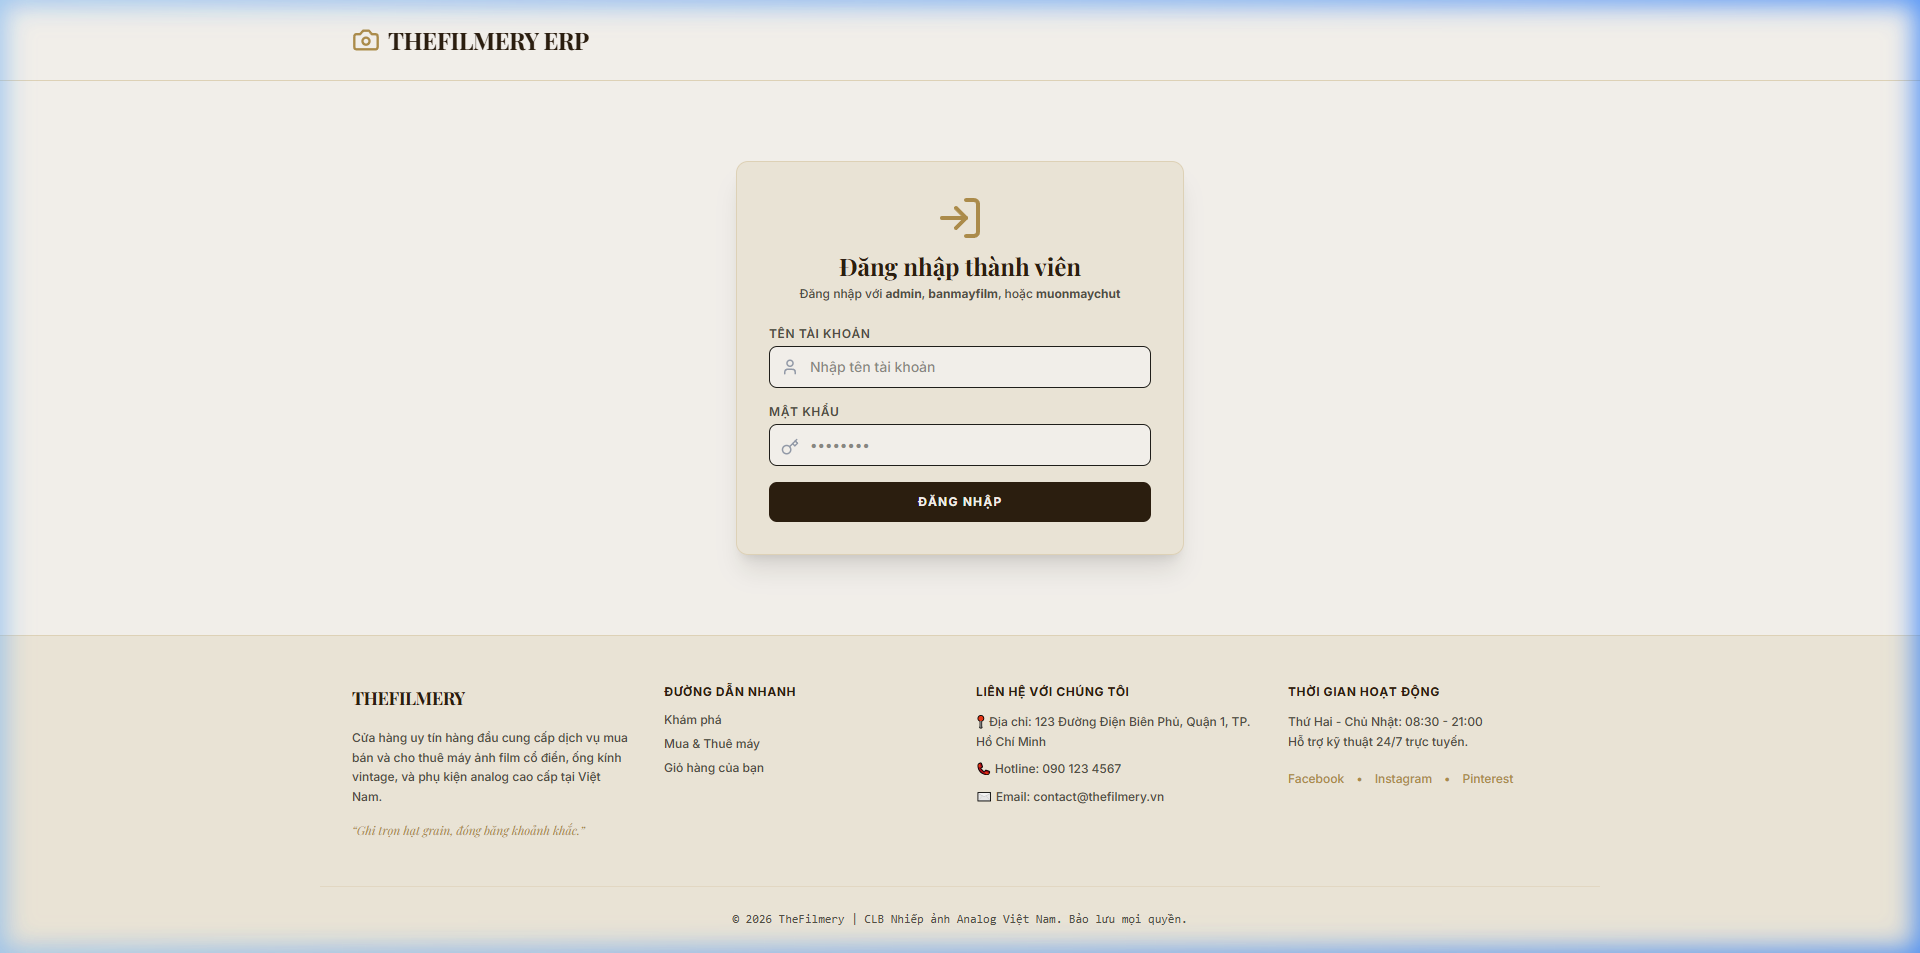
\includegraphics[width=0.85\textwidth]{Images/GiaoDien/login_page.png}
	\caption{Giao diện Đăng nhập hệ thống}
	\label{fig:login}
\end{figure}

Giao diện Đăng nhập phục vụ cho tất cả các tác nhân trong hệ thống gồm Admin, Nhân viên cho thuê và Nhân viên bán hàng. Giao diện này hiện thực UC02 - Đăng nhập hệ thống.

Người dùng nhập email/tên đăng nhập và mật khẩu. Sau khi bấm nút đăng nhập, frontend gửi request tới API đăng nhập của backend. Backend xác thực thông tin qua Supabase Auth, sau đó truy vấn bảng \texttt{users} để lấy vai trò và trạng thái tài khoản. Nếu tài khoản hợp lệ và đang hoạt động, hệ thống trả về access token và điều hướng người dùng tới màn hình tương ứng với vai trò.

\begin{table}[H]
	\centering
	\begin{tabularx}{\textwidth}{|l|X|}
		\hline
		\textbf{Thành phần} & \textbf{Nội dung} \\
		\hline
		Actor & Admin, NHANVIENTHUE, NHANVIENBAN \\
		\hline
		Use Case & UC02 \\
		\hline
		API & \texttt{POST /api/auth/login} \\
		\hline
		Bảng dữ liệu & \texttt{users}, Supabase Auth \\
		\hline
		Kết quả & Đăng nhập thành công và phân quyền giao diện \\
		\hline
	\end{tabularx}
\end{table}

% ------------------------------
\subsubsection{Giao diện Tổng quan}
% ------------------------------

\begin{figure}[H]
	\centering
	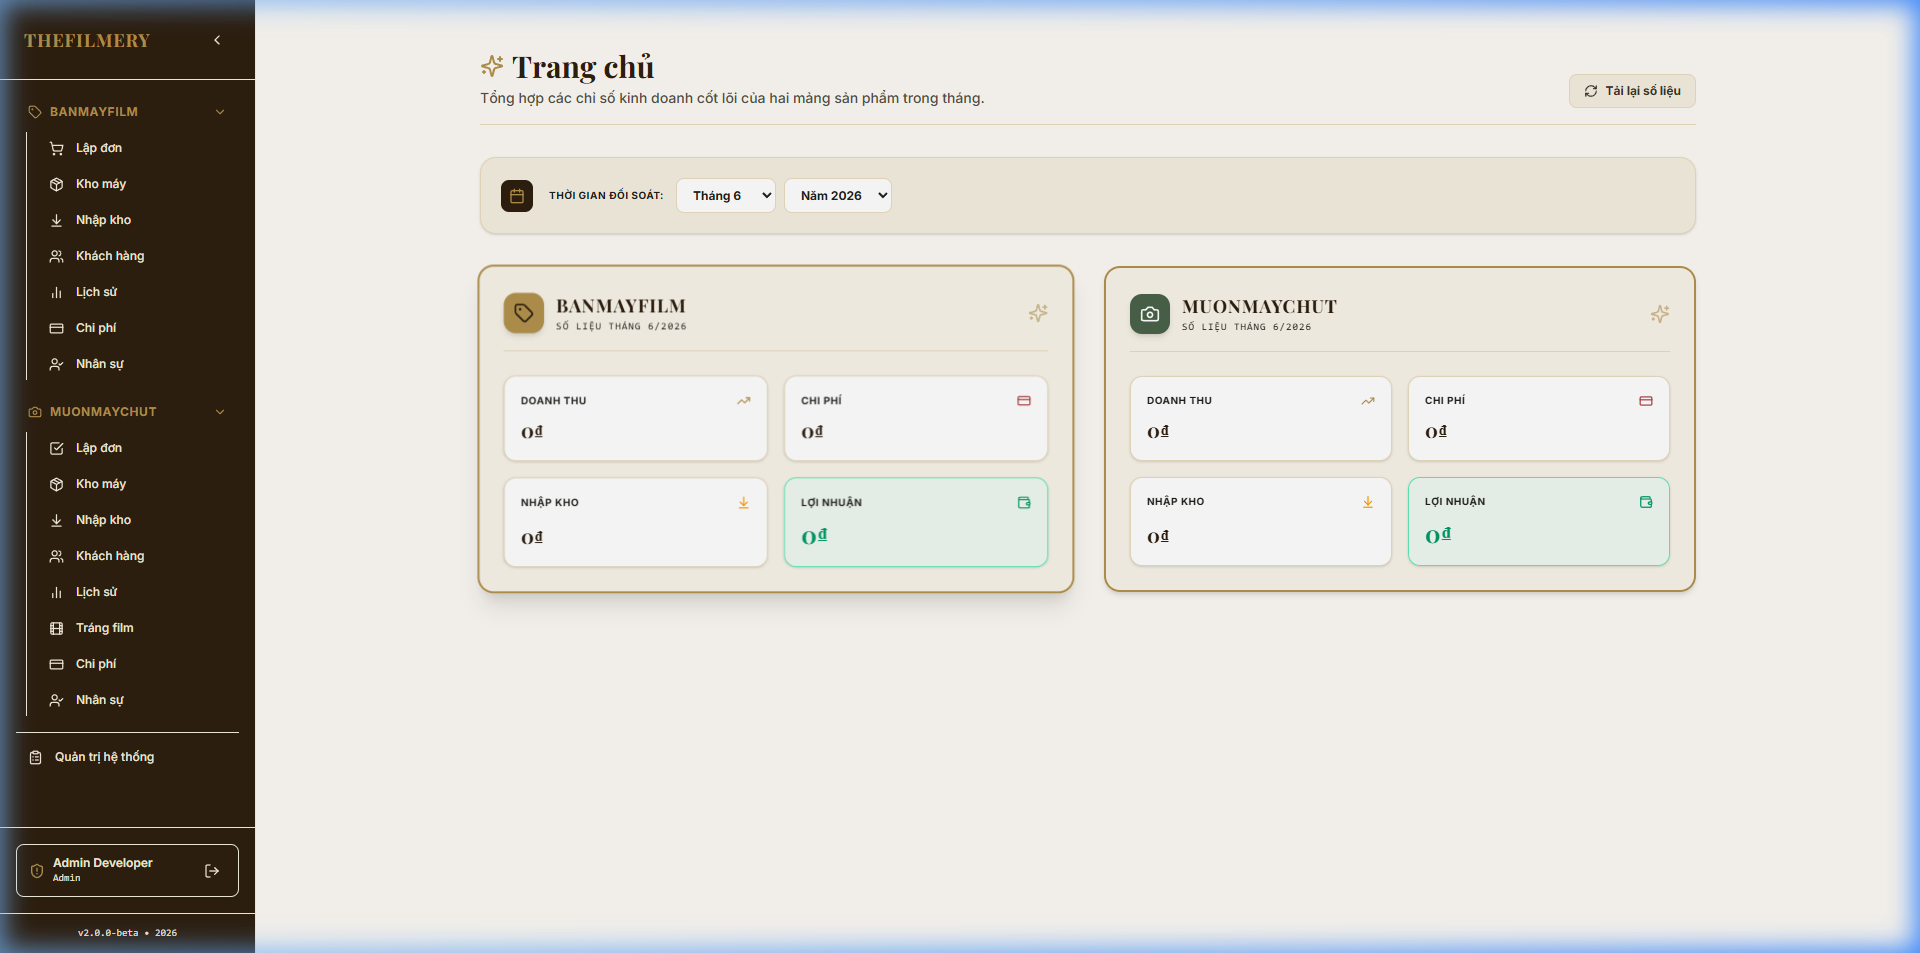
\includegraphics[width=0.95\textwidth]{Images/GiaoDien/admin_dashboard.png}
	\caption{Giao diện Tổng quan dành cho Admin}
	\label{fig:dashboard}
\end{figure}

Giao diện Tổng quan (Dashboard) phục vụ cho tác nhân Admin. Giao diện này hiện thực một phần các chức năng theo dõi và giám sát tổng quát. Giao diện hiển thị các thông tin tổng hợp, số liệu thống kê nhanh về tình hình kinh doanh, giúp quản trị viên nắm bắt trạng thái hệ thống.

\begin{table}[H]
	\centering
	\begin{tabularx}{\textwidth}{|l|X|}
		\hline
		\textbf{Thành phần} & \textbf{Nội dung} \\
		\hline
		Actor & Admin \\
		\hline
		Use Case & Tổng hợp thông tin thống kê \\
		\hline
		API & API thống kê tổng quan \\
		\hline
		Bảng dữ liệu & \texttt{transactions}, \texttt{bookings}, \texttt{sale\_orders} \\
		\hline
		Kết quả & Hiển thị số liệu tổng quát cho người quản trị \\
		\hline
	\end{tabularx}
\end{table}

% ------------------------------
\subsubsection{Giao diện Lập đơn thuê}
% ------------------------------

\begin{figure}[H]
	\centering
	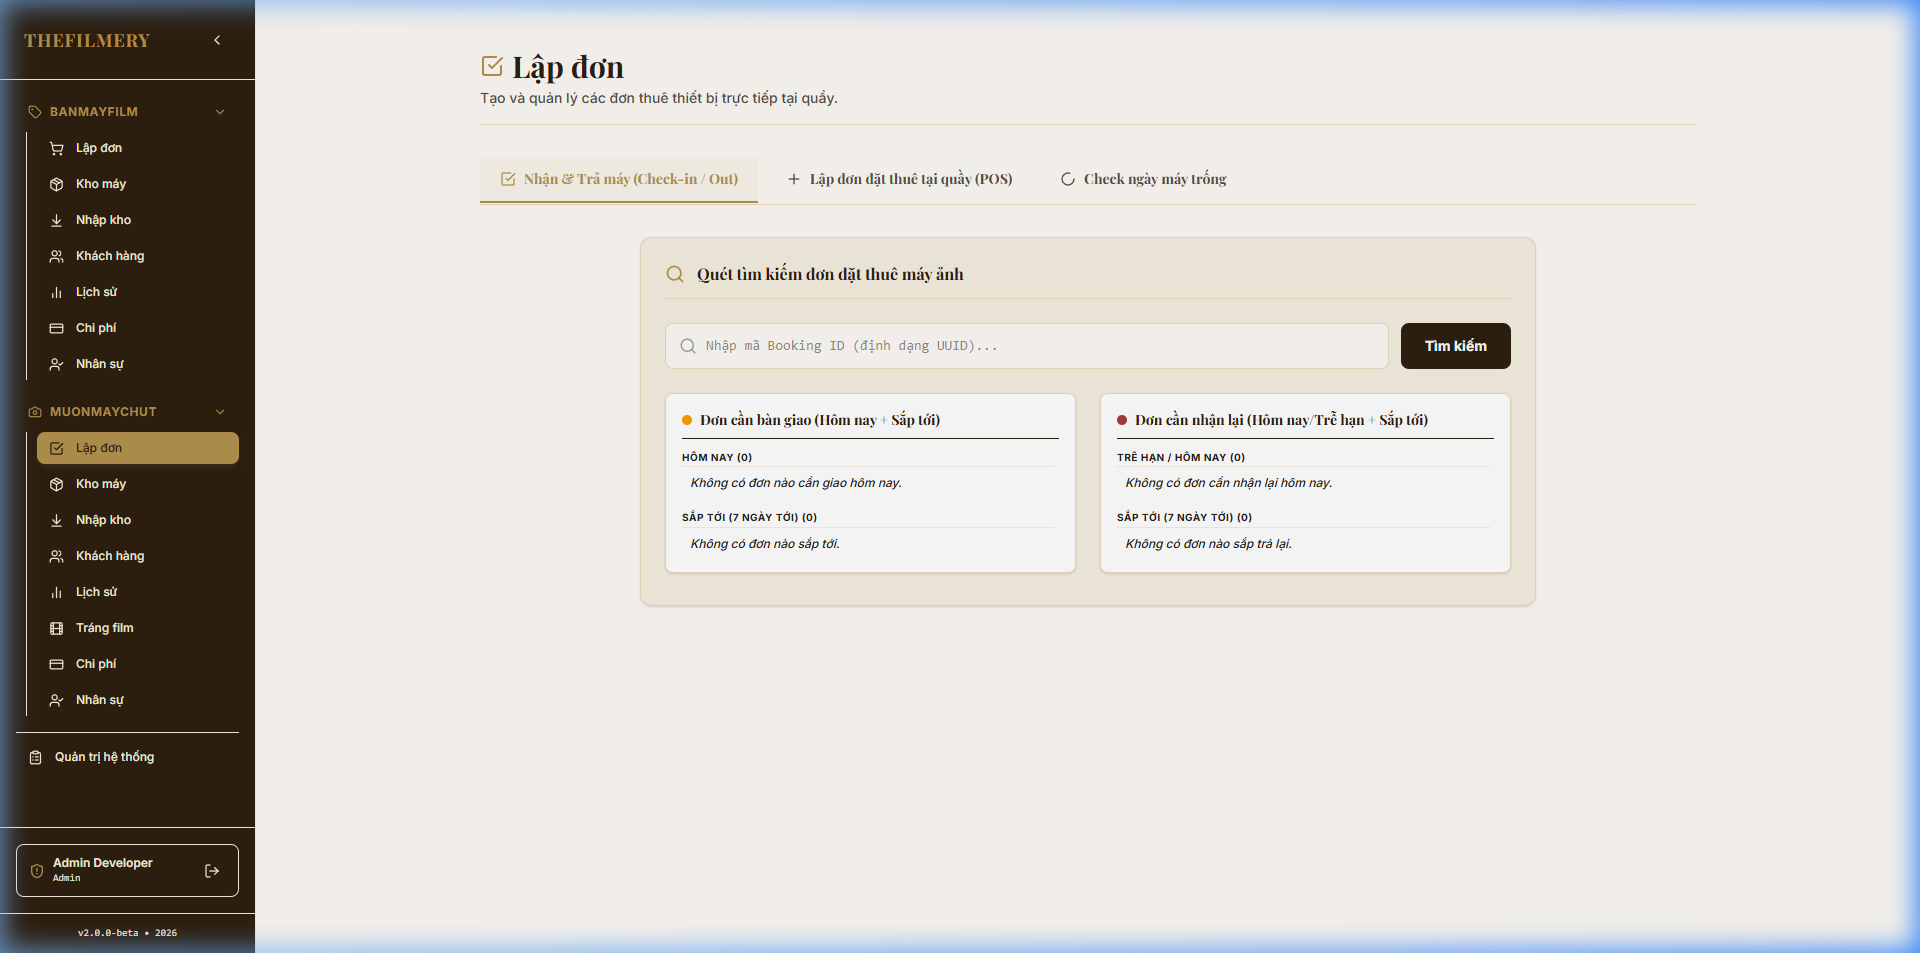
\includegraphics[width=0.95\textwidth]{Images/GiaoDien/rental_pos.png}
	\caption{Giao diện Lập đơn thuê máy (POS)}
	\label{fig:rental_pos}
\end{figure}

Giao diện Lập đơn thuê là giao diện trọng tâm của phân hệ cho thuê thiết bị, phục vụ tác nhân Nhân viên cho thuê. Giao diện này hiện thực các Use Case UC13 - Tạo đặt lịch thuê, UC14 - Check-in bàn giao, UC15 - Check-out quyết toán cọc, UC16 - Hủy booking và UC17 - Gia hạn thuê.

Khi tạo đơn thuê mới, nhân viên chọn khách hàng, dòng máy, thời gian thuê và các thông tin đặt cọc. Hệ thống kiểm tra tính hợp lệ của khoảng thời gian thuê, tìm thiết bị vật lý khả dụng không bị trùng lịch, sau đó tự động gán thiết bị cho booking. Sau khi tạo thành công, dữ liệu được ghi vào bảng \texttt{bookings} và \texttt{booking\_equipments}, đồng thời trạng thái thiết bị trong bảng \texttt{equipments} được cập nhật.

\begin{table}[H]
	\centering
	\begin{tabularx}{\textwidth}{|l|X|}
		\hline
		\textbf{Thành phần} & \textbf{Nội dung} \\
		\hline
		Actor & NHANVIENTHUE \\
		\hline
		Use Case & UC13, UC14, UC15, UC16, UC17 \\
		\hline
		API chính & \texttt{POST /api/bookings}, \texttt{POST /api/bookings/:id/checkin}, \texttt{POST /api/transactions/settle} \\
		\hline
		Bảng dữ liệu & \texttt{customers}, \texttt{camera\_models}, \texttt{equipments}, \texttt{bookings}, \texttt{booking\_equipments}, \texttt{transactions} \\
		\hline
		Kết quả & Tạo booking, bàn giao, nhận trả máy và quyết toán cọc \\
		\hline
	\end{tabularx}
\end{table}

% ------------------------------
\subsubsection{Giao diện Kho máy cho thuê}
% ------------------------------

\begin{figure}[H]
	\centering
	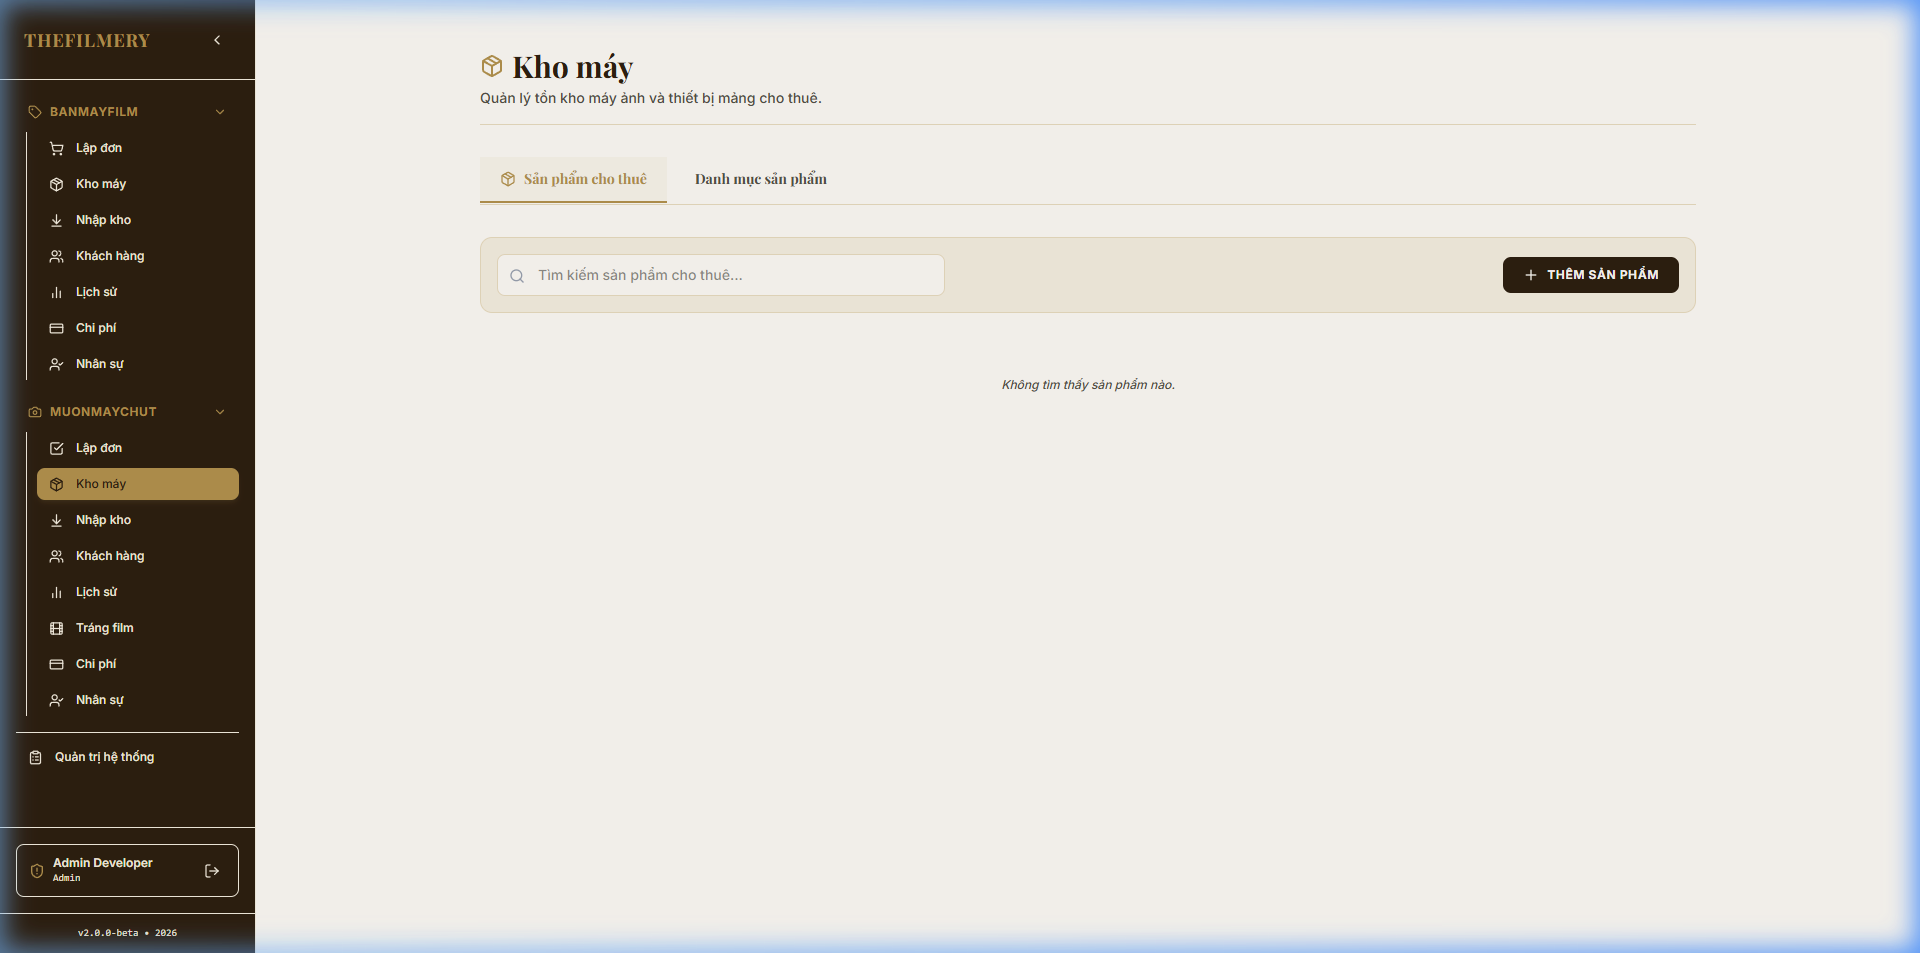
\includegraphics[width=0.95\textwidth]{Images/GiaoDien/rental_inventory.png}
	\caption{Giao diện Quản lý kho máy cho thuê}
	\label{fig:rental_inventory}
\end{figure}

Giao diện Kho máy cho thuê hiện thực các Use Case UC09 - Quản lý dòng máy ảnh thuê và UC10 - Quản lý thiết bị vật lý. Giao diện cho phép nhân viên xem danh sách dòng máy, tình trạng từng thiết bị theo serial number và cập nhật trạng thái thiết bị như AVAILABLE, RENTED, MAINTENANCE hoặc DAMAGED.

\begin{table}[H]
	\centering
	\begin{tabularx}{\textwidth}{|l|X|}
		\hline
		\textbf{Thành phần} & \textbf{Nội dung} \\
		\hline
		Actor & Admin, NHANVIENTHUE \\
		\hline
		Use Case & UC09, UC10 \\
		\hline
		API & API camera models, API equipments \\
		\hline
		Bảng dữ liệu & \texttt{camera\_models}, \texttt{equipments}, \texttt{maintenance\_logs} \\
		\hline
		Kết quả & Quản lý dòng máy và trạng thái thiết bị vật lý \\
		\hline
	\end{tabularx}
\end{table}

% ------------------------------
\subsubsection{Giao diện Lập đơn bán hàng}
% ------------------------------

\begin{figure}[H]
	\centering
	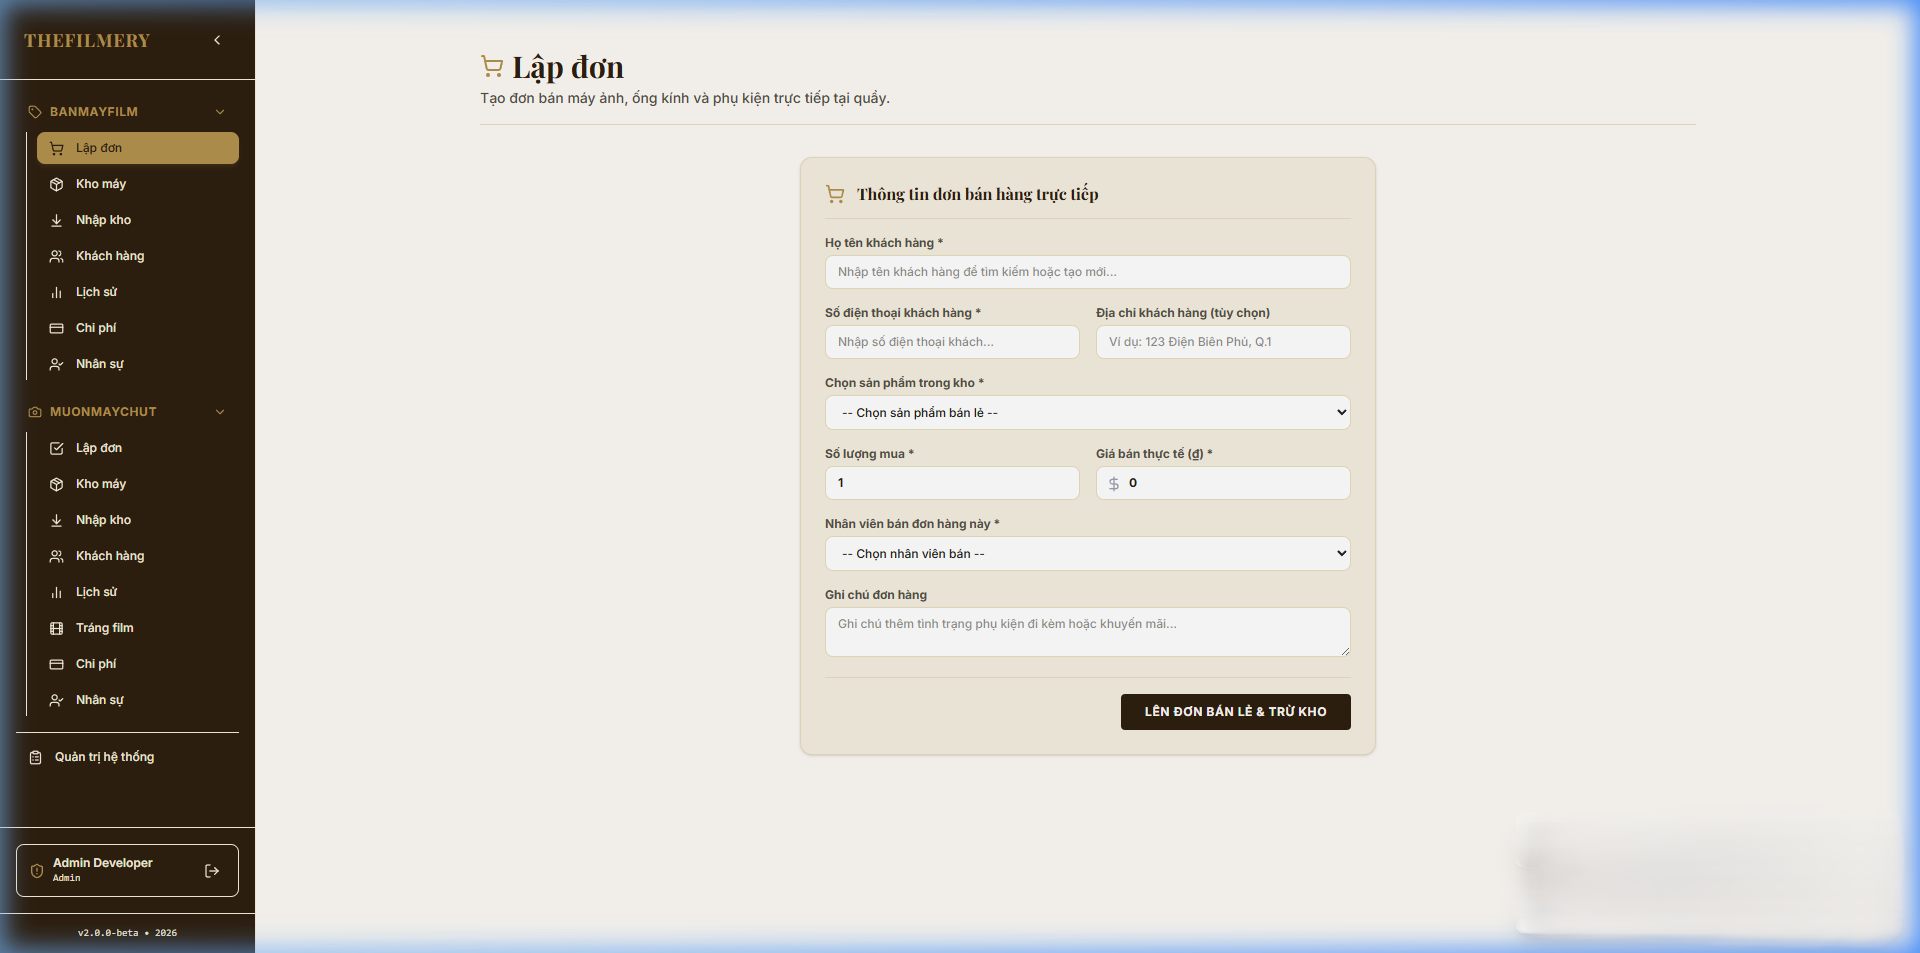
\includegraphics[width=0.95\textwidth]{Images/GiaoDien/sale_order_create.png}
	\caption{Giao diện Lập đơn bán hàng}
	\label{fig:sale_order}
\end{figure}

Giao diện Lập đơn bán hàng phục vụ tác nhân Nhân viên bán hàng. Giao diện này hiện thực UC21 - Tạo đơn bán hàng POS. Nhân viên chọn sản phẩm, nhập số lượng và xác nhận thanh toán. Hệ thống kiểm tra tồn kho của sản phẩm bán lẻ, tạo đơn bán hàng, cập nhật tồn kho và ghi nhận giao dịch tài chính tương ứng.

\begin{table}[H]
	\centering
	\begin{tabularx}{\textwidth}{|l|X|}
		\hline
		\textbf{Thành phần} & \textbf{Nội dung} \\
		\hline
		Actor & NHANVIENBAN \\
		\hline
		Use Case & UC21 \\
		\hline
		API & API tạo đơn bán hàng POS \\
		\hline
		Bảng dữ liệu & \texttt{sale\_products}, \texttt{sale\_orders}, \texttt{transactions} \\
		\hline
		Kết quả & Đơn bán được tạo, tồn kho giảm, giao dịch được ghi nhận \\
		\hline
	\end{tabularx}
\end{table}

% ------------------------------
\subsubsection{Giao diện Kho hàng bán}
% ------------------------------

\begin{figure}[H]
	\centering
	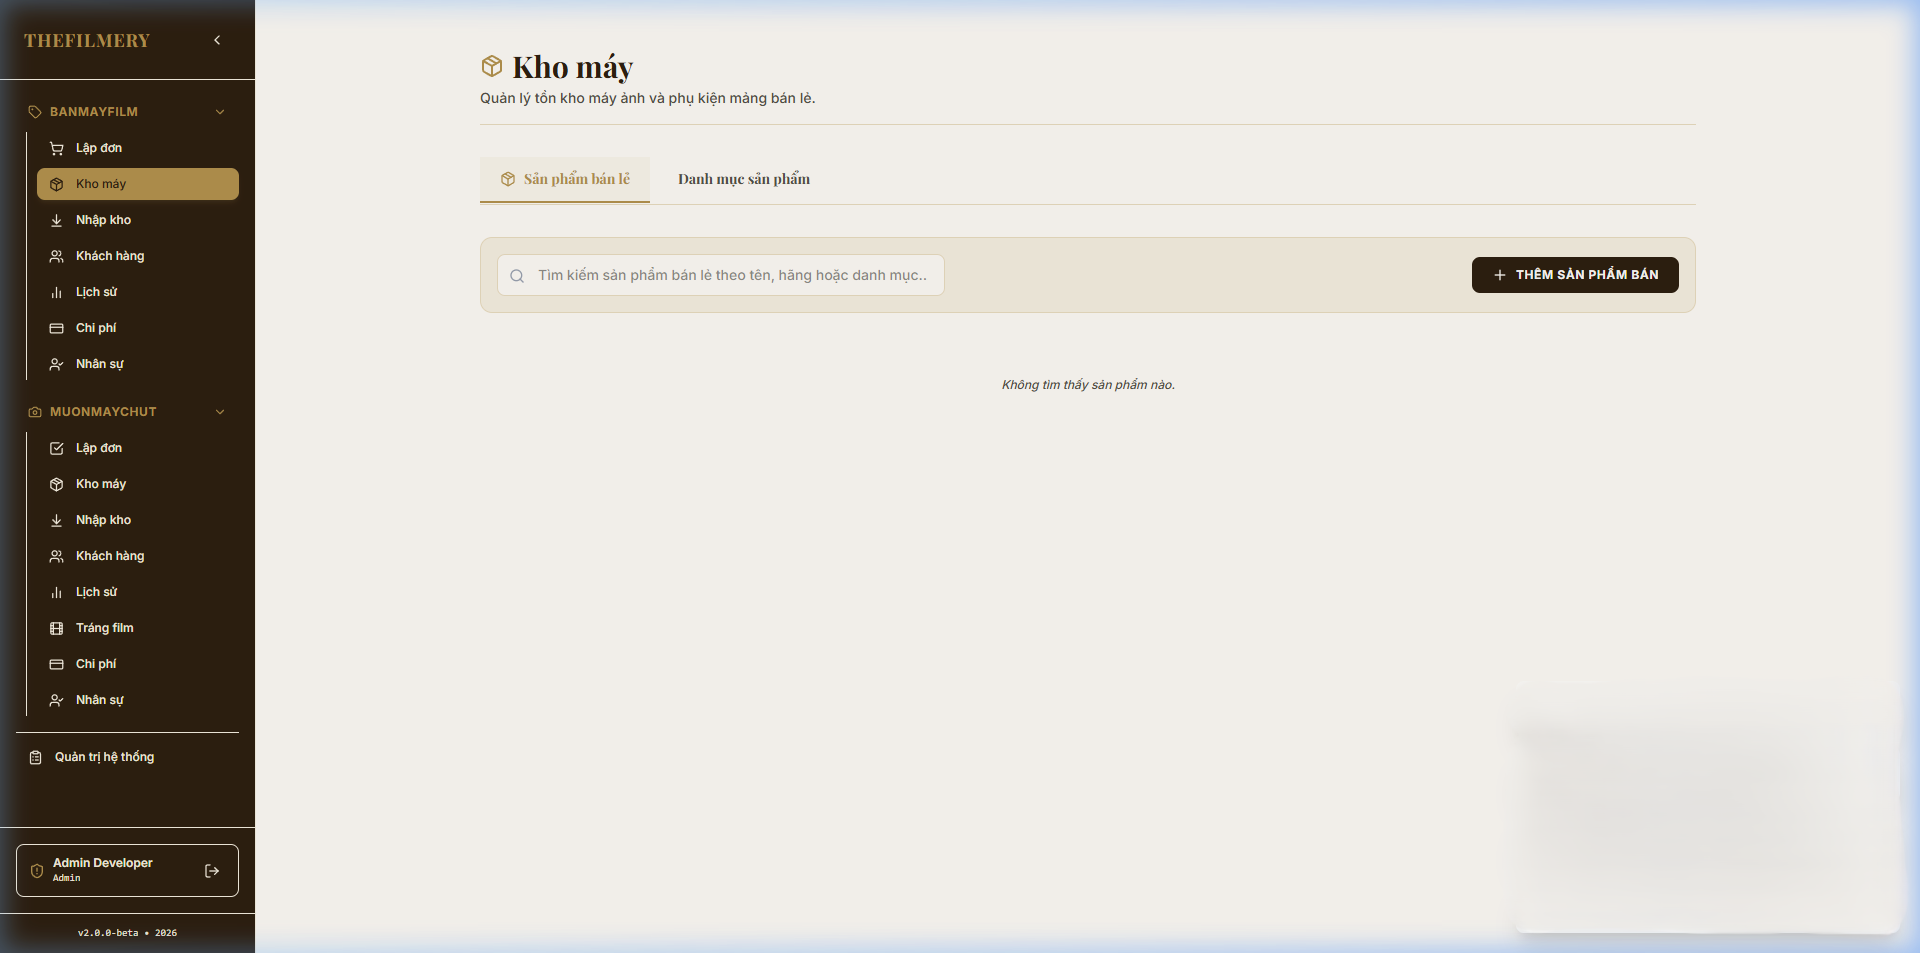
\includegraphics[width=0.95\textwidth]{Images/GiaoDien/sale_inventory.png}
	\caption{Giao diện Quản lý kho hàng bán}
	\label{fig:sale_inventory}
\end{figure}

Giao diện Kho hàng bán phục vụ tác nhân Admin và Nhân viên bán. Giao diện này hiện thực UC19 - Quản lý sản phẩm bán lẻ. Cho phép xem danh sách sản phẩm, quản lý số lượng tồn kho, giá bán và thông tin cơ bản của các mặt hàng bán lẻ.

\begin{table}[H]
	\centering
	\begin{tabularx}{\textwidth}{|l|X|}
		\hline
		\textbf{Thành phần} & \textbf{Nội dung} \\
		\hline
		Actor & Admin, NHANVIENBAN \\
		\hline
		Use Case & UC19 \\
		\hline
		API & API sale products \\
		\hline
		Bảng dữ liệu & \texttt{sale\_products} \\
		\hline
		Kết quả & Cập nhật và quản lý thông tin, tồn kho sản phẩm bán lẻ \\
		\hline
	\end{tabularx}
\end{table}

% ------------------------------
\subsubsection{Giao diện Khách hàng}
% ------------------------------

\begin{figure}[H]
	\centering
	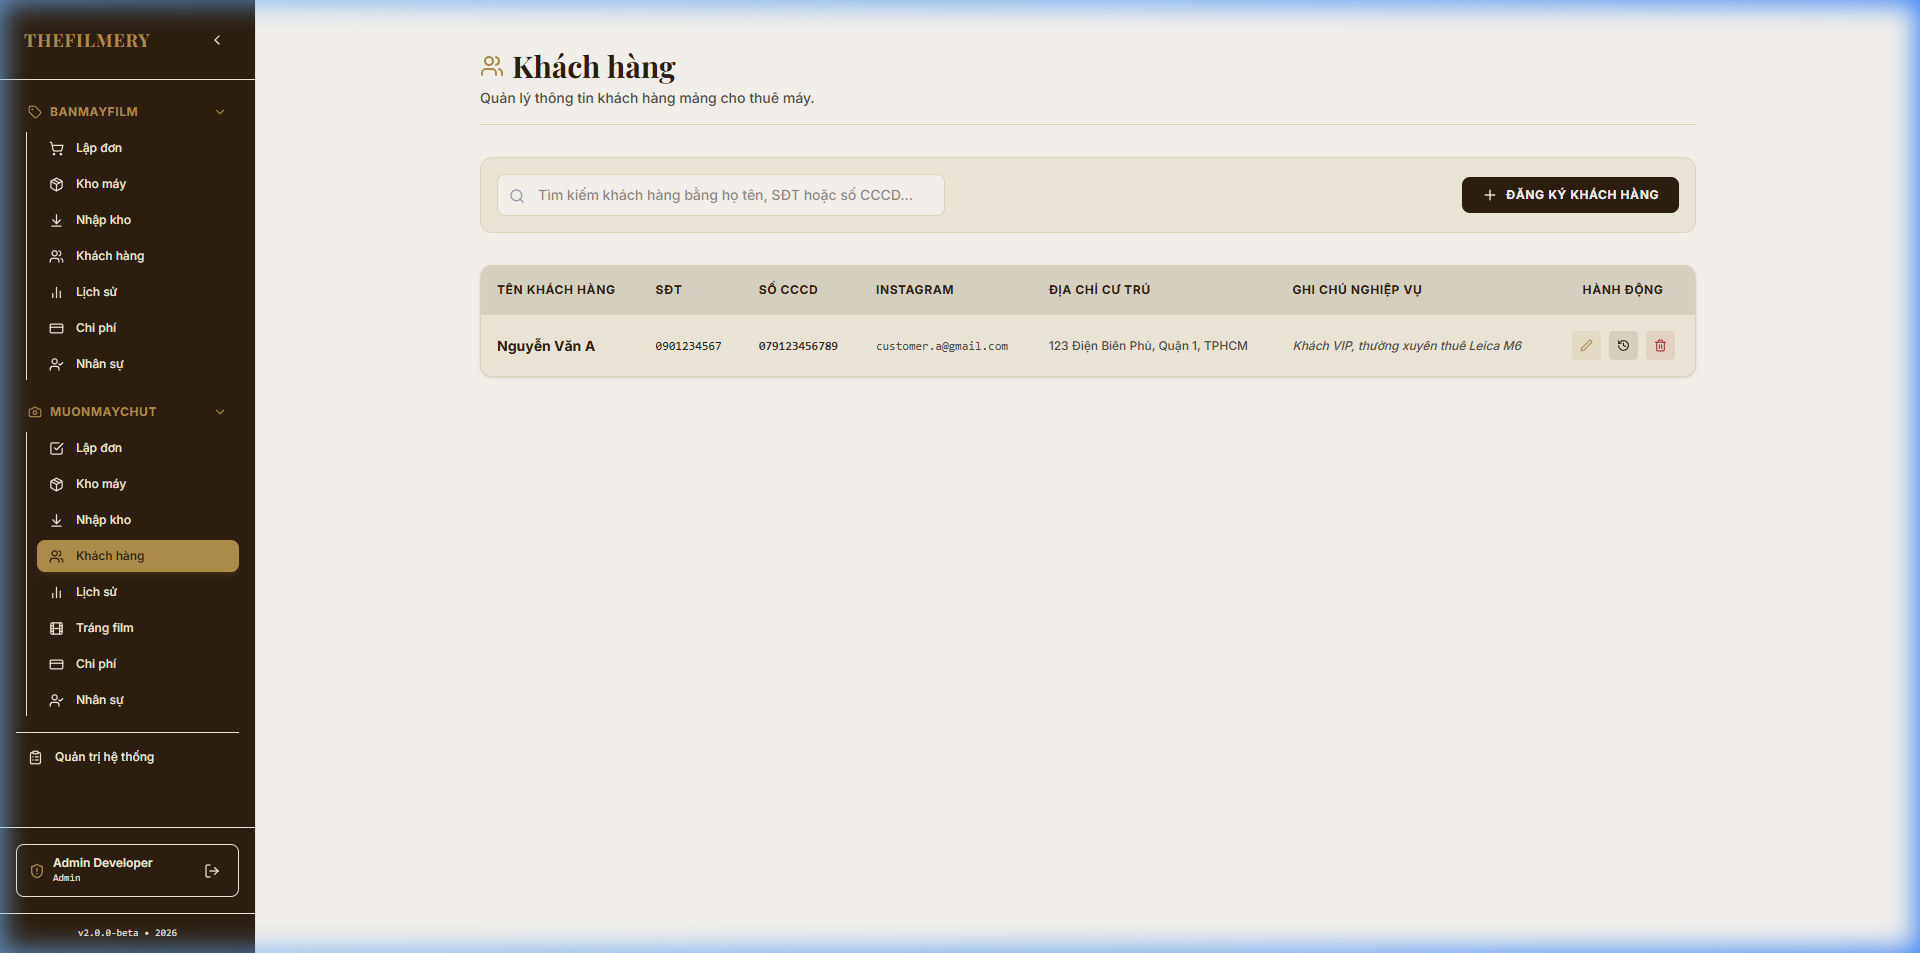
\includegraphics[width=0.95\textwidth]{Images/GiaoDien/rental_customers.png}
	\caption{Giao diện Quản lý khách hàng}
	\label{fig:rental_customers}
\end{figure}

Giao diện Khách hàng (áp dụng cho cả phân hệ bán và thuê) phục vụ tác nhân Nhân viên bán và Nhân viên thuê. Giao diện hiện thực UC22 và UC23 - Quản lý khách hàng mua/thuê. Cho phép lưu trữ và tra cứu thông tin khách hàng, lịch sử giao dịch và thông tin liên hệ.

\begin{table}[H]
	\centering
	\begin{tabularx}{\textwidth}{|l|X|}
		\hline
		\textbf{Thành phần} & \textbf{Nội dung} \\
		\hline
		Actor & NHANVIENBAN, NHANVIENTHUE \\
		\hline
		Use Case & UC22, UC23 \\
		\hline
		API & API sale customers, API rental customers \\
		\hline
		Bảng dữ liệu & \texttt{customers}, \texttt{sale\_customers} \\
		\hline
		Kết quả & Cập nhật hồ sơ khách hàng, xem lịch sử giao dịch \\
		\hline
	\end{tabularx}
\end{table}

% ------------------------------
\subsubsection{Giao diện Báo cáo}
% ------------------------------

\begin{figure}[H]
	\centering
	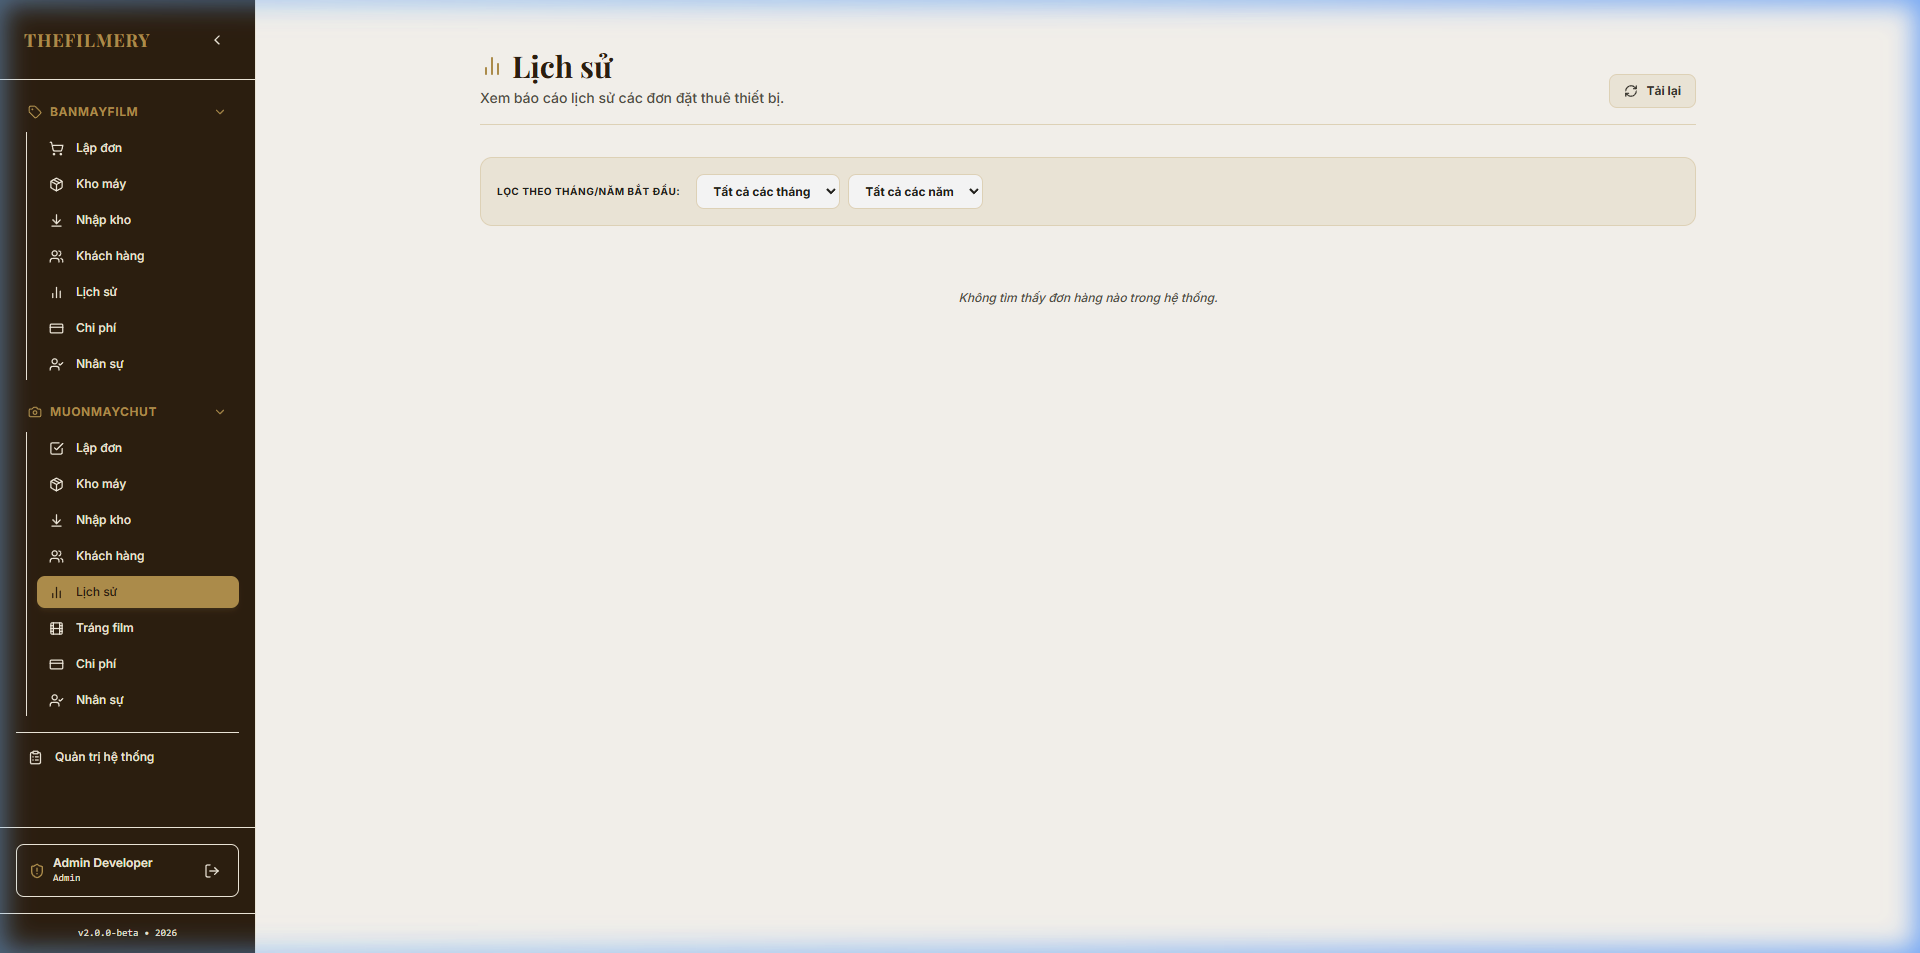
\includegraphics[width=0.95\textwidth]{Images/GiaoDien/rental_reporting.png}
	\caption{Giao diện Báo cáo}
	\label{fig:rental_reporting}
\end{figure}

Giao diện Báo cáo phục vụ tác nhân Admin. Hiện thực UC26 - Báo cáo doanh thu và UC27 - Lịch sử đơn hàng. Cung cấp các thống kê về doanh thu, chi phí, lợi nhuận theo các tiêu chí thời gian.

\begin{table}[H]
	\centering
	\begin{tabularx}{\textwidth}{|l|X|}
		\hline
		\textbf{Thành phần} & \textbf{Nội dung} \\
		\hline
		Actor & Admin \\
		\hline
		Use Case & UC26, UC27 \\
		\hline
		API & API reports, API history \\
		\hline
		Bảng dữ liệu & \texttt{transactions}, \texttt{bookings}, \texttt{sale\_orders} \\
		\hline
		Kết quả & Trích xuất và hiển thị dữ liệu báo cáo thống kê \\
		\hline
	\end{tabularx}
\end{table}

% ------------------------------
\subsubsection{Giao diện Quản trị hệ thống}
% ------------------------------

\begin{figure}[H]
	\centering
	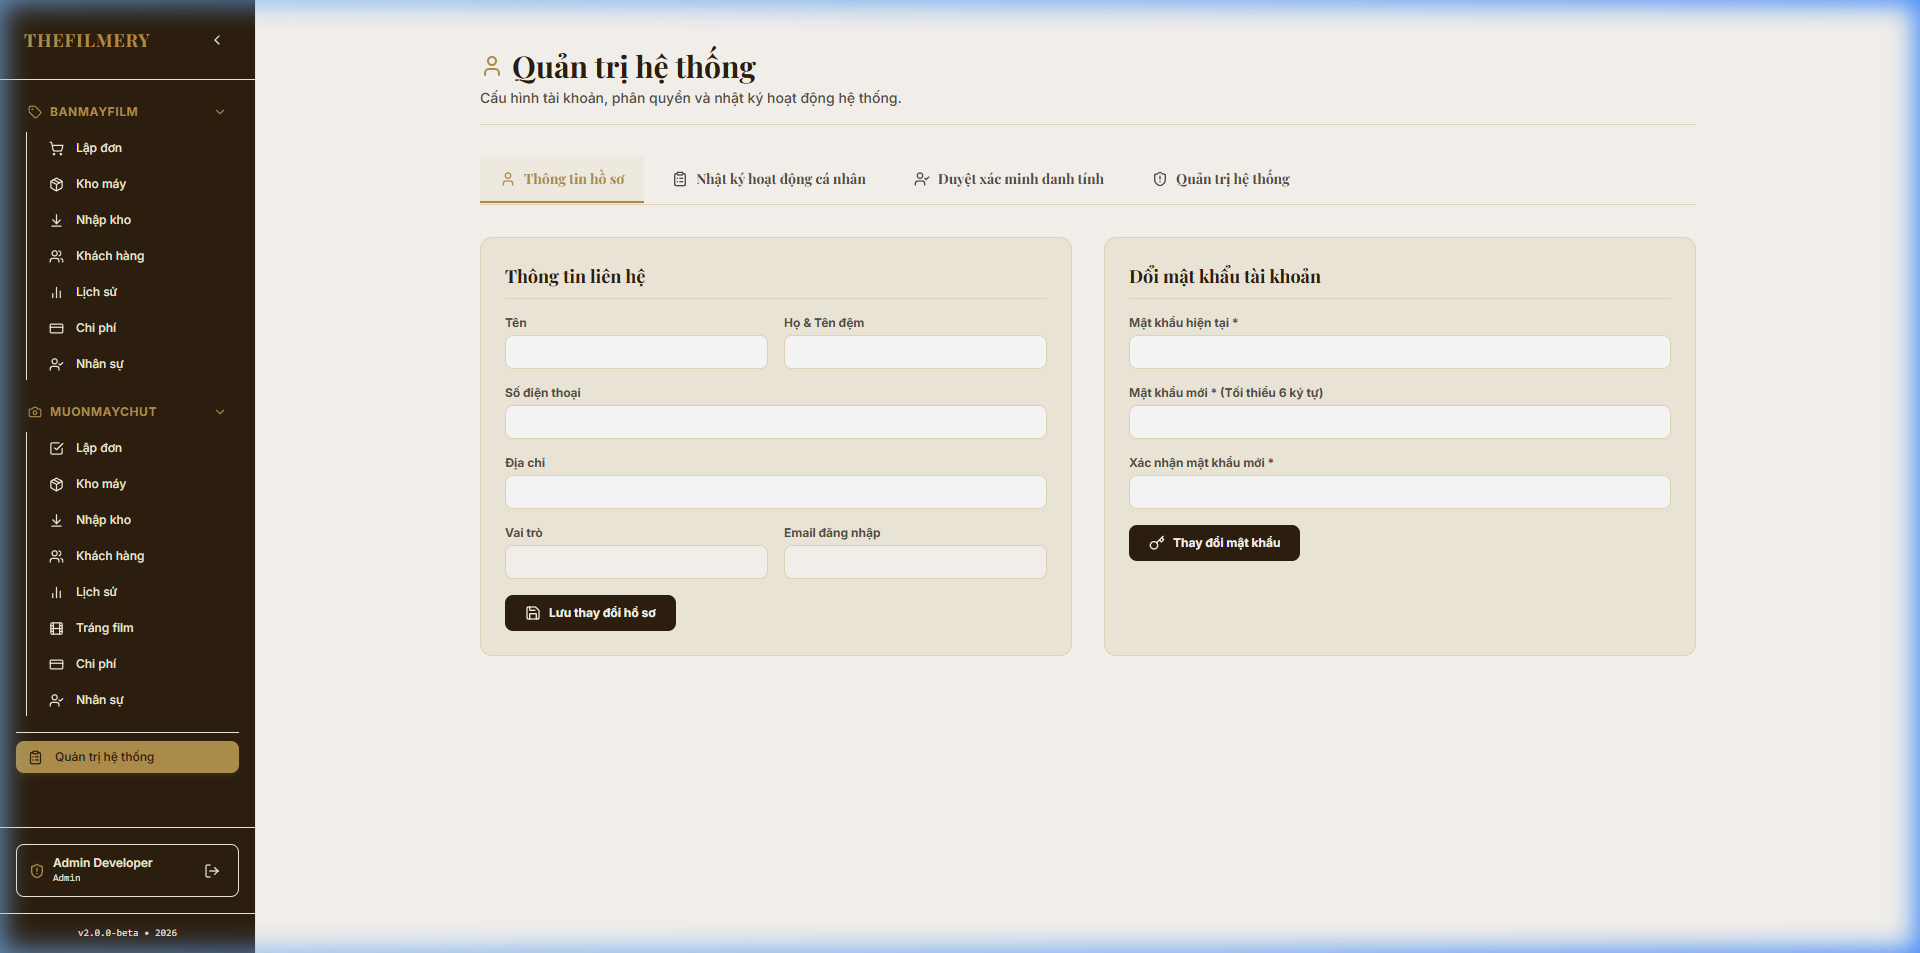
\includegraphics[width=0.95\textwidth]{Images/GiaoDien/profile_logs.png}
	\caption{Giao diện Quản trị hệ thống}
	\label{fig:profile_logs}
\end{figure}

Giao diện Quản trị hệ thống phục vụ tác nhân Admin. Hiện thực các Use Case liên quan đến quản lý tài khoản như UC01 - Đăng ký tài khoản nhân viên, UC04 - Kích hoạt/vô hiệu hóa tài khoản và quản lý thông tin hồ sơ nhân viên.

\begin{table}[H]
	\centering
	\begin{tabularx}{\textwidth}{|l|X|}
		\hline
		\textbf{Thành phần} & \textbf{Nội dung} \\
		\hline
		Actor & Admin \\
		\hline
		Use Case & UC01, UC04 \\
		\hline
		API & \texttt{PUT /api/auth/users/:id/status}, API users \\
		\hline
		Bảng dữ liệu & \texttt{users} \\
		\hline
		Kết quả & Quản lý danh sách, phân quyền và trạng thái tài khoản \\
		\hline
	\end{tabularx}
\end{table}


% ============================================================
\subsection{Chạy thử các Use Case chính}
% ============================================================

Nhóm tiến hành chạy thử các Use Case trọng tâm với dữ liệu đầu vào, thao tác thực hiện, kết quả mong đợi và kết quả thực tế.

% ------------------------------
\subsubsection{Kịch bản UC02 - Đăng nhập hệ thống}
% ------------------------------

\begin{table}[H]
	\centering
	\begin{tabularx}{\textwidth}{|l|X|}
		\hline
		\textbf{Thành phần} & \textbf{Nội dung} \\
		\hline
		Use Case & UC02 - Đăng nhập \\
		\hline
		Actor & Admin / Nhân viên \\
		\hline
		Tiền điều kiện & Tài khoản đã tồn tại và đang hoạt động \\
		\hline
		Dữ liệu đầu vào & Email/tên đăng nhập, mật khẩu \\
		\hline
		Thao tác & Nhập thông tin và bấm đăng nhập \\
		\hline
		Kết quả mong đợi & Hệ thống xác thực thành công, chuyển tới dashboard \\
		\hline
		Kết quả thực tế & Đăng nhập thành công, giao diện hiển thị theo vai trò \\
		\hline
		Trạng thái & Đạt \\
		\hline
	\end{tabularx}
\end{table}

Nhóm tiến hành kiểm thử UC02 bằng tài khoản thử nghiệm trong môi trường phát triển. Sau khi nhập thông tin đăng nhập hợp lệ, hệ thống gửi request xác thực tới backend. Backend kiểm tra thông tin qua Supabase Auth và truy vấn bảng \texttt{users} để lấy vai trò người dùng. Kết quả cho thấy người dùng đăng nhập thành công và được điều hướng tới giao diện phù hợp với quyền hạn.

% ------------------------------
\subsubsection{Kịch bản UC13 - Tạo đặt lịch thuê thiết bị}
% ------------------------------

\begin{table}[H]
	\centering
	\begin{tabularx}{\textwidth}{|l|X|}
		\hline
		\textbf{Thành phần} & \textbf{Nội dung} \\
		\hline
		Use Case & UC13 - Tạo đặt lịch thuê thiết bị \\
		\hline
		Actor & NHANVIENTHUE \\
		\hline
		Tiền điều kiện & Nhân viên đã đăng nhập; khách hàng tồn tại; dòng máy còn thiết bị khả dụng \\
		\hline
		Dữ liệu đầu vào & Khách hàng, dòng máy, ngày thuê, ngày trả, tiền cọc \\
		\hline
		Thao tác & Nhân viên tạo booking mới \\
		\hline
		Kết quả mong đợi & Booking được tạo ở trạng thái \texttt{PENDING}; thiết bị rảnh được tự động gán \\
		\hline
		Bảng bị tác động & \texttt{bookings}, \texttt{booking\_equipments}, \texttt{equipments} \\
		\hline
		Kết quả thực tế & Hệ thống tạo đơn thuê và hiển thị trong danh sách \\
		\hline
		Trạng thái & Đạt \\
		\hline
	\end{tabularx}
\end{table}

Ở kịch bản UC13, nhân viên cho thuê nhập thông tin khách hàng, chọn dòng máy cần thuê và khoảng thời gian thuê. Khi xác nhận tạo đơn, hệ thống thực hiện kiểm tra xung đột lịch thuê bằng cách đối chiếu các bản ghi trong \texttt{booking\_equipments} và \texttt{bookings}. Nếu tìm được thiết bị vật lý khả dụng, hệ thống tạo bản ghi booking mới, tạo liên kết thiết bị trong \texttt{booking\_equipments} và cập nhật trạng thái thiết bị tương ứng. Kết quả chạy thử cho thấy đơn thuê được tạo thành công và xuất hiện trong danh sách lịch sử thuê.

\begin{table}[H]
	\centering
	\begin{tabularx}{\textwidth}{|X|X|}
		\hline
		\textbf{Trường hợp ngoại lệ} & \textbf{Kết quả mong đợi} \\
		\hline
		Chọn khoảng thời gian đã có thiết bị bị đặt hết & Hệ thống báo không còn thiết bị khả dụng \\
		\hline
		Ngày trả trước ngày thuê & Hệ thống báo dữ liệu không hợp lệ \\
		\hline
		Thiếu khách hàng & Hệ thống yêu cầu chọn khách hàng \\
		\hline
	\end{tabularx}
\end{table}

% ------------------------------
\subsubsection{Kịch bản UC14 - Check-in bàn giao thiết bị}
% ------------------------------

\begin{table}[H]
	\centering
	\begin{tabularx}{\textwidth}{|l|X|}
		\hline
		\textbf{Thành phần} & \textbf{Nội dung} \\
		\hline
		Use Case & UC14 - Check-in bàn giao thiết bị \\
		\hline
		Actor & NHANVIENTHUE \\
		\hline
		Tiền điều kiện & Booking đang ở trạng thái \texttt{PENDING} hoặc \texttt{CONFIRMED} \\
		\hline
		Dữ liệu đầu vào & Booking ID, phụ kiện bàn giao, tình trạng thiết bị \\
		\hline
		Thao tác & Nhân viên bấm Check-in \\
		\hline
		Kết quả mong đợi & Booking chuyển sang \texttt{CHECKED\_IN}, ghi nhận thời điểm bàn giao \\
		\hline
		Bảng bị tác động & \texttt{bookings}, \texttt{booking\_equipments}, \texttt{equipments} \\
		\hline
		Trạng thái & Đạt \\
		\hline
	\end{tabularx}
\end{table}

Với UC14, nhân viên chọn một đơn thuê đã được tạo và thực hiện thao tác Check-in. Hệ thống kiểm tra trạng thái hiện tại của booking, sau đó ghi nhận thời điểm bàn giao, nhân viên bàn giao và tình trạng thiết bị khi giao đi. Thông tin phụ kiện kèm theo được lưu vào bản ghi liên kết giữa booking và thiết bị. Sau khi xử lý thành công, đơn thuê chuyển sang trạng thái \texttt{CHECKED\_IN}.

% ------------------------------
\subsubsection{Kịch bản UC15 - Check-out và quyết toán cọc}
% ------------------------------

\begin{table}[H]
	\centering
	\begin{tabularx}{\textwidth}{|l|X|}
		\hline
		\textbf{Thành phần} & \textbf{Nội dung} \\
		\hline
		Use Case & UC15 - Check-out / Tất toán \\
		\hline
		Actor & NHANVIENTHUE \\
		\hline
		Tiền điều kiện & Booking đang ở trạng thái \texttt{CHECKED\_IN} \\
		\hline
		Dữ liệu đầu vào & Giờ trả, tình trạng hư hỏng, phí hư hỏng, ghi chú \\
		\hline
		Thao tác & Nhân viên xác nhận trả máy \\
		\hline
		Kết quả mong đợi & Tính tiền thuê, phụ phí, tiền hoàn cọc; thiết bị về \texttt{AVAILABLE} \\
		\hline
		Bảng bị tác động & \texttt{bookings}, \texttt{transactions}, \texttt{equipments} \\
		\hline
		Trạng thái & Đạt \\
		\hline
	\end{tabularx}
\end{table}

Ở kịch bản UC15, nhân viên thực hiện nhận lại thiết bị từ khách hàng và nhập thông tin trả máy. Hệ thống tính tiền thuê cơ bản dựa trên số ngày thuê, kiểm tra giờ trả thực tế để tính phụ phí quá giờ nếu có, đồng thời khấu trừ phí hư hỏng vào tiền cọc. Sau khi tất toán, booking được cập nhật trạng thái \texttt{CHECKED\_OUT}, thiết bị vật lý được đưa về trạng thái \texttt{AVAILABLE} và giao dịch hoàn cọc hoặc khấu trừ được ghi nhận trong bảng \texttt{transactions}.

\begin{table}[H]
	\centering
	\begin{tabularx}{\textwidth}{|l|X|}
		\hline
		\textbf{Giờ trả thực tế} & \textbf{Kết quả xử lý} \\
		\hline
		Trước hoặc bằng 22:00 & Không tính phụ phí \\
		\hline
		22:01 - 22:30 & Phụ thu 50\% đơn giá thuê ngày \\
		\hline
		Sau 22:30 & Phụ thu 100\% đơn giá thuê ngày \\
		\hline
	\end{tabularx}
\end{table}

% ------------------------------
\subsubsection{Kịch bản UC21 - Tạo đơn bán hàng POS}
% ------------------------------

\begin{table}[H]
	\centering
	\begin{tabularx}{\textwidth}{|l|X|}
		\hline
		\textbf{Thành phần} & \textbf{Nội dung} \\
		\hline
		Use Case & UC21 - Tạo đơn bán hàng POS \\
		\hline
		Actor & NHANVIENBAN \\
		\hline
		Tiền điều kiện & Nhân viên đã đăng nhập; sản phẩm còn tồn kho \\
		\hline
		Dữ liệu đầu vào & Sản phẩm, số lượng, phương thức thanh toán \\
		\hline
		Thao tác & Nhân viên tạo đơn bán \\
		\hline
		Kết quả mong đợi & Đơn bán được tạo, tồn kho giảm, giao dịch được ghi nhận \\
		\hline
		Bảng bị tác động & \texttt{sale\_orders}, \texttt{sale\_products}, \texttt{transactions} \\
		\hline
		Trạng thái & Đạt \\
		\hline
	\end{tabularx}
\end{table}

Trong kịch bản UC21, nhân viên bán hàng chọn sản phẩm bán lẻ, nhập số lượng và xác nhận thanh toán. Hệ thống kiểm tra tồn kho khả dụng của sản phẩm. Nếu số lượng tồn kho đủ, hệ thống tạo đơn bán hàng, cập nhật tồn kho và ghi nhận giao dịch doanh thu. Nếu tồn kho không đủ, hệ thống hiển thị thông báo lỗi và không tạo đơn.

\begin{table}[H]
	\centering
	\begin{tabularx}{\textwidth}{|X|X|}
		\hline
		\textbf{Trường hợp ngoại lệ} & \textbf{Kết quả mong đợi} \\
		\hline
		Số lượng bán lớn hơn tồn kho & Không cho tạo đơn, báo thiếu hàng \\
		\hline
		Chưa chọn sản phẩm & Báo thiếu thông tin \\
		\hline
		Thanh toán thất bại & Không ghi nhận đơn hoàn tất \\
		\hline
	\end{tabularx}
\end{table}

% ------------------------------
\subsubsection{Kịch bản UC26 - Xem báo cáo doanh thu}
% ------------------------------

\begin{table}[H]
	\centering
	\begin{tabularx}{\textwidth}{|l|X|}
		\hline
		\textbf{Thành phần} & \textbf{Nội dung} \\
		\hline
		Use Case & UC26 - Báo cáo doanh thu \\
		\hline
		Actor & Admin \\
		\hline
		Tiền điều kiện & Admin đã đăng nhập \\
		\hline
		Dữ liệu đầu vào & Khoảng thời gian lọc \\
		\hline
		Thao tác & Chọn ngày/tháng/năm và xem báo cáo \\
		\hline
		Kết quả mong đợi & Hệ thống hiển thị doanh thu thuê, doanh thu bán, chi phí, lợi nhuận \\
		\hline
		Bảng dữ liệu & \texttt{transactions}, \texttt{bookings}, \texttt{sale\_orders}, \texttt{expenses} \\
		\hline
		Trạng thái & Đạt \\
		\hline
	\end{tabularx}
\end{table}

Ở kịch bản UC26, quản trị viên truy cập giao diện báo cáo và chọn khoảng thời gian cần thống kê. Hệ thống tổng hợp dữ liệu từ các giao dịch thuê máy, bán hàng POS và chi phí vận hành để hiển thị doanh thu, chi phí và lợi nhuận tương ứng. Kết quả chạy thử cho thấy báo cáo được cập nhật theo bộ lọc thời gian và hỗ trợ quản lý theo dõi tình hình kinh doanh.

% ------------------------------
\subsubsection{Tổng hợp kết quả chạy thử}
% ------------------------------

\begin{table}[H]
	\centering
	\caption{Tổng hợp kết quả chạy thử các Use Case chính}
	\begin{tabularx}{\textwidth}{|l|l|X|l|}
		\hline
		\textbf{UC} & \textbf{Tên Use Case} & \textbf{Kết quả} & \textbf{Ghi chú} \\
		\hline
		UC02 & Đăng nhập & Đạt & Phân quyền thành công \\
		\hline
		UC13 & Tạo booking & Đạt & Cần kiểm thử thêm trường hợp nhiều người đặt đồng thời \\
		\hline
		UC14 & Check-in & Đạt & Cập nhật trạng thái bàn giao thành công \\
		\hline
		UC15 & Check-out & Đạt & Cần kiểm tra thêm các mốc phụ phí \\
		\hline
		UC21 & POS & Đạt & Cần thống nhất schema đơn nhiều sản phẩm \\
		\hline
		UC26 & Báo cáo doanh thu & Đạt & Hiển thị dữ liệu chính xác theo mốc thời gian \\
		\hline
	\end{tabularx}
\end{table}


% ============================================================
\subsection{Đánh giá kết quả hiện thực hóa}
% ============================================================

Qua quá trình hiện thực hóa và chạy thử các Use Case chính, hệ thống đã bước đầu đáp ứng các yêu cầu nghiệp vụ cốt lõi đã phân tích. Các luồng quan trọng như đăng nhập, tạo booking, bàn giao thiết bị, tất toán trả máy, tạo đơn bán hàng POS và xem báo cáo doanh thu đã được cài đặt và kiểm thử ở mức chức năng.

Kết quả chạy thử cho thấy mô hình kiến trúc 3 tầng được áp dụng nhất quán: frontend đảm nhiệm giao diện tương tác, backend xử lý logic nghiệp vụ và database lưu trữ dữ liệu. Các thao tác nghiệp vụ chính đều có sự thay đổi dữ liệu tương ứng trong các bảng liên quan, thể hiện sự liên kết giữa thiết kế cơ sở dữ liệu ở Chương 4 và phần cài đặt thực tế.

Tuy nhiên, việc kiểm thử hiện tại chủ yếu tập trung vào các kịch bản chức năng cơ bản. Hệ thống vẫn cần được bổ sung kiểm thử tự động, kiểm thử đồng thời đối với nghiệp vụ đặt lịch thuê và kiểm thử tải để đánh giá độ ổn định khi vận hành thực tế.

\cleardoublepage